%!TEX program = xelatex
\documentclass[11pt,a4paper]{article}
\usepackage[utf8]{inputenc}
\usepackage[T1]{fontenc}
\usepackage{authblk}
\usepackage{tikz}
\usepackage{pgfplots}
\usepackage{verbatim}
\usepackage{amsfonts}
\usepackage{amsmath}
\usepackage{amsthm}
\usepackage{indentfirst}
\usepackage{amssymb}
\usepackage{enumerate}
\linespread{1.6}
\setlength{\footskip}{20pt}
\setlength{\parindent}{0pt}
\usetikzlibrary{shapes,snakes}
\newcommand{\argmax}{\operatornamewithlimits{argmax}}
\newcommand{\argmin}{\operatornamewithlimits{argmin}}
\DeclareMathOperator{\col}{col}
\usepackage{booktabs}
\newtheorem{theorem}{Theorem}
\newtheorem{note}{Note}
\newtheorem{definition}{Definition}
\newtheorem{proposition}{Proposition}
\newtheorem{lemma}{Lemma}
\newtheorem{example}{Example}
\newtheorem{corollary}{Corollary}
\usepackage{graphicx}
\usepackage{geometry}
\usepackage{hyperref}
\newcommand{\code}{	exttt}
\geometry{a4paper,scale=0.8}
\title{Notes of Probability}
\author[*]{Wenxiao Yang}
\affil[*]{Department of Mathematics, University of Illinois at Urbana-Champaign}
\date{Last updated: 2022.09}


\begin{document}
\maketitle
\tableofcontents
\newpage

\section{Distribution}

\subsection{Discrete}
\subsubsection{Bernoulli Distribution -- $\operatorname{Bernoulli}(\pi)$: an event happens with probability $\pi$}
Assume $n$ independent binary (taking values $0$ or $1$) observations arising from independent and identical trials: $y_{1}, y_{2}, \ldots, y_{n}$ such that: $P\left(Y_{i}=1\right)=\pi$ and $P\left(Y_{i}=0\right)=1-\pi$.

Random variables $Y_{i}$ are normally called \textbf{Bernoulli} trials, $Y_{i} \sim \operatorname{Bernoulli}(\pi)$. $$\mathbb{E}(Y_i)=\pi,Var(Y_i)=\pi(1-\pi)$$

\subsubsection{Binomial distribution -- $bin(n,\pi)$: $n$ independent Bernoulli distributions}
The random variable $Y=\sum_{i=1}^{n} Y_{i}$ has the Binomial distribution with index $n$ and parameter $\pi$ denoted as $Y \sim \operatorname{bin}(n, \pi)$.
Mass probability function for $Y$ :
$$
P(y)=\left(\begin{array}{l}
n \\
y
\end{array}\right) \pi^{y}(1-\pi)^{n-y}
$$
with $\left(\begin{array}{l}n \\ y\end{array}\right)=\frac{n !}{y !(n-y) !}$ and $y=0,1,2, \ldots, n$
\begin{enumerate}[(1)]
    \item Mean and Variance:
    $\mathbb{E}(Y)=\mu=n \pi,\operatorname{Var}(Y)=\sigma^{2}=n \pi(1-\pi)$
    \item Skewness: $\mathbb{E}\frac{(Y-\mu)^{3}}{\sigma^{3}}=\frac{1-2 \pi}{\sqrt{n \pi(1-\pi)}}$
    \item If the independence assumption is violated, the Binomial distribution does not apply.
    \item Normal approximation:$\frac{Y-n \pi}{\sqrt{n \pi(1-\pi)}} \stackrel{d}{\longrightarrow} N(0,1),\quad {n \rightarrow \infty}$.
\end{enumerate}

\subsubsection{Multinomial Distribution}

\subsubsection{Poisson Distribution -- $Pois(\lambda)$: an event happens $k$ times within unit time}
$\lambda$: frequency of the event, i.e., the average number of event happens within unit time.
$$\Pr(X{=}k)= \frac{\lambda^k e^{-\lambda}}{k!},\ k=0,1,2,3...$$
$$E(X)=Var(X)=\lambda$$

\subsubsection*{Derivation process:}
Consider a unit time (the unit is divided into $n$ equal subparts, $n \rightarrow \infty$), there is an event may occur with every subpart, the number of the event happens should follow binomial distribution $B(n,p)$. where $n \rightarrow \infty, p \rightarrow 0$; $\lambda=n\cdot p$ is the expected number of events in this period of time.

the probability the number of the event happens:
\begin{equation}
    \begin{aligned}
        \Pr(X=k)&=\lim_{n \rightarrow\infty} \binom{n}{k} (\frac{\lambda}{n})^k(1-\frac{\lambda}{n})^{n-k}\\
        &=\lim_{n \rightarrow\infty} \frac{n!}{(n-k)!k!} (\frac{\lambda}{n})^k(1-\frac{\lambda}{n})^{n}(1-\frac{\lambda}{n})^{-k}\\
        &=\lim_{n \rightarrow\infty}\frac{n!}{(n-k)!k!} (\frac{\lambda}{n})^k e^{-\lambda}\\
        &=\frac{\lambda^k e^{-\lambda}}{k!}\lim_{n \rightarrow\infty}\frac{n!}{(n-k)!n^k}\\
        &=\frac{\lambda^k e^{-\lambda}}{k!}\lim_{n \rightarrow\infty}
        \frac{n}{n}\frac{n-1}{n}\cdots \frac{n-k+1}{n}\\
        &=\frac{\lambda^k e^{-\lambda}}{k!}
    \end{aligned}
    \nonumber
\end{equation}

\subsubsection*{Sums of independent Poisson random variables are Poisson random variables}
$X\sim Pois(\lambda_1), Y\sim Pois(\lambda_2)$ are two independent Poisson random variables, then $Z=X+Y$ also follow Poisson distribution, and the paramenter is the sum of $X$'s and $Y$'s
\begin{equation}
    \begin{aligned}
        Z\sim Pois(\lambda_1+\lambda_2)
    \end{aligned}
    \nonumber
\end{equation}
Then, $$Z=X_1+X_2+\cdots+X_n\sim Pois(\lambda_1+\lambda_2+\cdots+\lambda_n)$$

\subsection{Continuous}
\subsubsection{Exponential distribution $Exp(\lambda)$: interval between to independent identical event / the first time a event happened}
$\lambda$: frequency of the event.

$X$ follows exponential distribution with parameter $\lambda$ or $\beta$:
$${\displaystyle X\sim {\text{Exp}}(\lambda )} \text{ or } {\displaystyle X\sim {\text{Exp}}(\beta )}$$
They are equivlanet, the only difference is $\beta=\frac{1}{\lambda}$.
$${f(x;{\lambda})=\left\{{\begin{matrix}{\lambda }e^{-{\lambda }x}&x\geq 0\\0&\;x<0.\end{matrix}}\right.}$$
$${f(x;{\beta})=\left\{{\begin{matrix}{\frac{1}{\beta} }e^{-{\frac{1}{\beta} }x}&x\geq 0\\0&\;x<0.\end{matrix}}\right.}$$
c.d.f is:
$${F(x;{\lambda})=\left\{{\begin{matrix}{1-}e^{-{\lambda }x}&x\geq 0\\0&\;x<0.\end{matrix}}\right.}$$
Note that $\lambda > 0$ is the frequcy of the occurance of the event; $\beta>0$ is the probability of the event happens in each second. The range of exponential distribution is $[0,\infty)$.

$\mathbb{E}(X)=\frac{1}{\lambda}$; $Var(X)=\frac{1}{\lambda^2}$
$$\mathbb{E}(X)=\frac{1}{\lambda};\ Var(X)=\frac{1}{\lambda^2}$$
Memorylessness: ${\displaystyle \Pr \left(T>s+t\mid T>s\right)=\Pr(T>t)}$
\begin{equation}
    \begin{aligned}
        \Pr (T>s+t\mid T>s)&=\frac{\Pr(T>s+t\text{ and }T>s)}{\Pr(T>s)}\\
        &=\frac{\Pr(T>s+t)}{\Pr(T>s)}\\
        &=\frac{e^{-\lambda(s+t)}}{e^{-\lambda s}}\\
        &=e^{-\lambda t}\\
        &=\Pr (T>t)
    \end{aligned}
    \nonumber
\end{equation}

\subsubsection*{Derivation process:}

Consider a unit time (the unit is divided into $n$ equal subparts, $n \rightarrow \infty$), there is an event may occur with every subpart, the number of the event happens should follow binomial distribution $B(n,p)$. where $n \rightarrow \infty, p \rightarrow 0$; $\lambda=n\cdot p$ is the expected number of events in this period of time. (the same as Poisson)\\
CDF:
\begin{equation}
    \begin{aligned}
        1-F(x;\lambda)=\lim_{n \rightarrow \infty}(1-\frac{\lambda}{n})^{nx}=e^{-\lambda x}
        \Rightarrow F(x;\lambda)=1-e^{-\lambda x}
    \end{aligned}
    \nonumber
\end{equation}
PDF:
\begin{equation}
    \begin{aligned}
        f(x;\lambda)=\frac{\partial F(x;\lambda)}{\partial x}=\lambda e^{-\lambda x}
    \end{aligned}
    \nonumber
\end{equation}

\subsubsection{Gaussian/Normal Distribution}
$N(\mu,\sigma^2)$. p.d.f. ${\displaystyle f(x)={\frac {1}{\sigma {\sqrt {2\pi }}}}e^{-{\frac {1}{2}}\left({\frac {x-\mu }{\sigma }}\right)^{2}}}$
\begin{theorem}
Suppose $X\sim N(\mu_1,\sigma_1^2)$ and $Y\sim N(\mu_2,\sigma_2^2)$ are independent, then $X+Y\sim N(\mu_1+\mu_2,\sigma_1^2+\sigma^2)$.
\end{theorem}
\begin{proof}
The MGF of $X$ is
\begin{equation}
    \begin{aligned}
        M_X(t)=\mathbb{E}e^{tx}&=\int_{-\infty}^{\infty}e^{tx}\frac{1}{\sqrt{2\pi}\sigma_1}e^{-\frac{(x-\mu_1)^2}{2\sigma_1^2}}dx\\
        &=\int_{-\infty}^{\infty}\frac{1}{\sqrt{2\pi}\sigma_1}e^{-\frac{x^2-2(\mu_1+\sigma_1^2t)x+\mu_1^2}{2\sigma_1^2}}dx\\
        &=e^{\frac{\sigma_1^4t^2+2\mu_1\sigma^2t}{2\sigma_1^2}}\int_{-\infty}^{\infty}\frac{1}{\sqrt{2\pi}\sigma_1}e^{-\frac{(x-(\mu_1+\sigma_1^2t))^2}{2\sigma_1^2}}dx\\
        &=e^{t\mu_1+\frac{1}{2}\sigma_1^2t^2}
    \end{aligned}
    \nonumber
\end{equation}
Then, the MGF of $X+Y$ is
\begin{equation}
    \begin{aligned}
        M_{X+Y}(t)=\mathbb{E}e^{t(X+Y)}=\mathbb{E}e^{tX}\mathbb{E}e^{tY}=e^{t(\mu_1+\mu_2)+\frac{1}{2}(\sigma_1^2+\sigma_2^2)t^2}=M_{Z}(t)
    \end{aligned}
    \nonumber
\end{equation}
where $Z\sim N(\mu_1+\mu_2,\sigma_1^2+\sigma^2)$
\end{proof}

\subsubsection{Multivariate/Joint Gaussian/Normal Distribution (MVN)}
A $k$-dimensional random vector $(X_1,X_2,...,X_k)^T=\mathbf{X}\sim N(\mu,\Sigma)$.

p.d.f. $${\displaystyle f_{\mathbf {X} }(x_{1},\ldots ,x_{k})={\frac {\exp \left(-{\frac {1}{2}}({\mathbf {x} }-{\boldsymbol {\mu }})^{\mathrm {T} }{\boldsymbol {\Sigma }}^{-1}({\mathbf {x} }-{\boldsymbol {\mu }})\right)}{\sqrt {(2\pi )^{k}|{\boldsymbol {\Sigma }}|}}}}$$

A random vector is said to be $k$-variate normally distributed if every linear combination of its $k$ components has a univariate normal distribution.
\begin{enumerate}[(1)]
    \item $\mu$ is a $k$-dimensional \textbf{mean vector}: $$\mu=\mathbb{E}[\mathbf{X}]=(\mathbb{E}[X_1],\mathbb{E}[X_2],...,\mathbb{E}[X_k])^T$$
    \item $\Sigma$ is a $k\times k$ \textbf{covariance matrix}$${\displaystyle \Sigma _{i,j}=\operatorname {E} [(X_{i}-\mu _{i})(X_{j}-\mu _{j})]=\operatorname {Cov} [X_{i},X_{j}]}$$
    \item The inverse of $\Sigma$, ${\boldsymbol {Q}}={\Sigma }^{-1}$ is \textbf{precision matrix}.
\end{enumerate}
\begin{theorem}
    MVN distribution is completely specified by knowing $\mu$, $\Sigma$.
\end{theorem}
\begin{proof}
MGF: $M_X(t_1,t_2,...,t_k)=\mathbb{E}e^{\sum_{i=1}^k t_ix_i}$

Since any linear combination of $X$ is also normal distribution, $\Omega=\sum_{i=1}^k t_ix_i$ follows normal distribution.
$$M_X(t_1,t_2,...,t_k)=\mathbb{E}e^\Omega=e^{\mathbb{E}(\Omega)+\frac{1}{2}Var(\Omega)}=e^{\sum_{i=1}^kt_i \mathbb{E}(x_i)+\frac{1}{2}Var(\sum_{i=1}^k t_ix_i)}$$
\end{proof}

Generally, "independence" is a \textbf{stronger} condition than "$0$ correlation" ($Cov=0$).
\begin{theorem}
    For \textbf{MVN}, "independence" is \textbf{equivalent} to "$0$ correlation"
\end{theorem}
\begin{proof}
As we show $M_X(t_1,t_2,...,t_k)=e^{\sum_{i=1}^kt_i \mathbb{E}(x_i)+\frac{1}{2}Var(\sum_{i=1}^k t_ix_i)}$. If $Cov(x_i,x_j)=0,\forall i,j\in S$,
\begin{equation}
    \begin{aligned}
        M_X(t_1,t_2,...,t_k)&=e^{\sum_{i=1}^kt_i \mathbb{E}(x_i)+\frac{1}{2}Var(\sum_{i=1}^k t_ix_i)}\\
        &=e^{\sum_{i=1}^it_ki \mathbb{E}(x_i)+\frac{1}{2}\sum_{i=1}^it_i^2Var(x_i)}\\
        &=\prod_{i=1}^ke^{t_i\mathbb{E}(x_i)+\frac{1}{2}t_i^2Var(x_i)}\\
        &=\prod_{i=1}^kM_{x_i}(t_i)
    \end{aligned}
    \nonumber
\end{equation}
\end{proof}

\begin{theorem}
    Independent $X=[X_1,X_2,...,X_n]\sim$ MVN and $Y=[Y_1,Y_2,...,Y_m]\sim$ MVN, then $W=[X_1,X_2,...,X_n,Y_1,Y_2,...,Y_m]\sim$ MVN.
\end{theorem}

\begin{theorem}
    Independent $X=[X_1,X_2,...,X_n]\sim N(\mu_1,\Sigma_1)$ and $Y=[Y_1,Y_2,...,Y_n]\sim N(\mu_2,\Sigma_2)$, then $X+Y\sim N(\mu_1+\mu_2,\Sigma_1+\Sigma_2)$.
\end{theorem}














\subsection{Poisson process: A sequence of arrivals in continuous time with rate $\lambda$}
\subsubsection{Definition}
$N(t)\sim Pois(\lambda t)$: Number of arrivals in length $t$ follows Poisson distribution
\begin{equation}
    \begin{aligned}
        N(t)\sim Pois(\lambda t)\\
        \Pr(N(t)=k)=\frac{(\lambda t)^k e^{-\lambda t}}{k!}
    \end{aligned}
    \nonumber
\end{equation}
The number of arrivals in disjoint time intervals are independent.
\subsubsection{$T_j$: time of $j^{th}$ arrival}
$T_1>t$ is same as $N(t)=0$: $P(T_1>t)=P(N(t)=0)=e^{-\lambda t}$\\
$\Rightarrow T_1\sim Expo(\lambda) \Rightarrow T_j-T_{j-1}\sim Expo(\lambda); T_j\sim Gamma(j,\lambda)$

\subsubsection{Theorem (Conditional counts): $N(t_1)|N(t_2)=n\sim Bin(n,\frac{t_1}{t_2})$}
(We can interpret the theorem as: $n$ points distribute uniformly in $(0,t_2]$, so the probability a point loctae within $(0,t_1]$ is $\frac{t_1}{t_2}$)

\section{Basis}
\subsection{Covariance and Variance}
\begin{enumerate}[(1)]
    \item $\sigma_{XY}=Cov(X,Y)=\mathbb{E}\left[(X-\mathbb{E}X)(Y-\mathbb{E}Y)\right]=\mathbb{E}(XY)-\mathbb{E}X\mathbb{E}Y$
    \item $Cov(aX+b,Y)=aCov(X,Y)$
    \item $Cov(X+Y,W)=Cov(X,W)+Cov(Y,W)$
    \item $Cov(aX+bY,cX+dY)=ac\ {Var}(X)+(ad+bc)Cov(X,Y)+bd\ {Var}(Y)$
    \item $Var(aX+bY)=a^2\ {Var}(X)+2ab\ Cov(X,Y)+b^2\ {Var}(Y)$
\end{enumerate}
\subsection{Conditional Expectation and Variance}
\begin{enumerate}[(1)]
    \item Conditional variance: $$Var(Y|X=x)=\mathbb{E}\left((Y-\mathbb{E}(Y|X=x))^2|X=x\right)
    =\mathbb{E}(Y^2|X=x)-(\mathbb{E}(Y|X=x))^2$$
    \item \textbf{Law of Total Expectation:} $$\mathbb{E}(Y)=\sum_{i=1}^n \mathbb{E}(Y|A_i)P(A_i)$$
    \item \textbf{Law of Iterated Expectation (Adam's Law):}
    $$\mathbb{E}\left[\mathbb{E}(Y|X)\right]=\mathbb{E}(Y)$$
    \item \textbf{Adam's Law with extra conditioning:} $$\mathbb{E}\left(\mathbb{E}(Y|X,Z)|Z\right)=\mathbb{E}(Y|Z)$$
    \item \textbf{Law of Total Variance:}$$Var(Y)=\mathbb{E}(Var(Y|X))+Var(\mathbb{E}(Y|X))$$
\end{enumerate}

\subsection{Gambler's Ruin}
Suppose a gambler at each round either wins a dollar or loses a dollar with probability $\frac{1}{2}$ each. Suppose the gambler starts at $k$ dollars. He stops when either he reaches his goal of $N$ dollars or he goes bankrupt and loses all his money.

Let $A$ be the event that the gambler is ruined.
\begin{equation}
    \begin{aligned}
        P(A|x=k)=\frac{1}{2}P(A|x=k-1)+\frac{1}{2}P(A|x=k+1)\\
        \Rightarrow p_k-p_{k-1}=p_{k+1}-p_k
    \end{aligned}
    \nonumber
\end{equation}
According to the setting, $p_0=1,p_N=0$, then $p_k=\frac{N-k}{N}$.

\subsection{Moment Generating Function (MGF)}
Let $X$ be a random variable. The moment generating function (mgf) of $X$, denoted by $M_X(t)$:
\begin{equation}
    \begin{aligned}
        \underline{M_X(t)=\mathbb{E}[e^{tX}]}=\mathbb{E}\left[1+tX+\frac{(tX)^2}{2!}+\frac{(tX)^3}{3!}+\cdots\right]=\sum_{n=0}^\infty\frac{\mathbb{E}[X^n]t^n}{n!}
    \end{aligned}
    \nonumber
\end{equation}
We can find $\frac{\partial M_X(t)}{\partial t}= \mathbb{E}\left[Xe^{tX}\right]$, then $\frac{\partial M_X(0)}{\partial t}= \mathbb{E}\left[X\right]$. More generally, we can find that $$\frac{\partial^n M_X(0)}{\partial t^n}= \mathbb{E}\left[X^n\right],n=1,2,...$$
\subsubsection*{Why MGF is useful?}
\begin{enumerate}[(1)]
    \item If $X,Y$ are independent, then $$M_{X+Y}(t)=\mathbb{E}[e^{(X+Y)t}]=\mathbb{E}[e^tX]\mathbb{E}[e^tY]=M_X(t)M_Y(t)$$
    \item Unique random variable (RV) $\Leftrightarrow$ unique MGF
\end{enumerate}

\subsection{Inequality}
\subsubsection{Cauchy-Schwarz inequality: $|\mathbb{E}XY|\leq \sqrt{\mathbb{E}X^2\cdot \mathbb{E}Y^2}$}
For any r.vs. $X$ and $Y$ with finite variance: $|\mathbb{E}XY|\leq \sqrt{\mathbb{E}X^2\cdot \mathbb{E}Y^2}$
\begin{example}[Second Moment Method]
$X$ is a non-negative r.v. We want to find an \underline{upper bound} on $P(X=0)$.
\end{example}
Because $X$ is non-negative, $X=X\cdot \textbf{I}_{X>0}=\left\{\begin{matrix}
    X,&X>0\\
    0,&X=0
\end{matrix}\right.$. Hence,
\begin{equation}
    \begin{aligned}
        \mathbb{E}X= \mathbb{E}X\cdot \textbf{I}_{X>0}\leq \sqrt{\mathbb{E} X^2\cdot \textbf{I}^2_{X>0}}=\sqrt{\mathbb{E}X^2}\sqrt{P(X>0)}\\
        \Rightarrow P(X>0)\geq\frac{(\mathbb{E}X)^2}{\mathbb{E}X^2} \Rightarrow P(X=0)=1-P(X>0)\leq \frac{Var(X)}{\mathbb{E}X^2}
    \end{aligned}
    \nonumber
\end{equation}

\subsubsection{Jensen's Inequality: convex $g$ $\Rightarrow$ $\mathbb{E}(g(X))\geq g(\mathbb{E}(X))$}
If $g$ is convex $\mathbb{E}(g(X))\geq g(\mathbb{E}X)$; If $g$ is concave $\mathbb{E}(g(X))\leq g(\mathbb{E}X)$.

\subsubsection{Markov's Inequality: $P(|X|\geq a)\leq \frac{\mathbb{E}|X|}{a}$}
For any r.v. $X$ and a constant $a>0$. $P(|X|\geq a)\leq \frac{\mathbb{E}|X|}{a}$
\begin{proof}
$Y=\frac{|X|}{a}$, $Y\geq \mathbb{I}_{Y\geq 1} \Rightarrow \mathbb{E}Y\geq P(Y\geq 1) \Rightarrow \frac{\mathbb{E}|X|}{a}\geq P(|X|\geq a)$
\end{proof}
\textbf{Note:} Markov's Inequality can also be written as $P(X\geq a)\leq \frac{\mathbb{E}X}{a}$, $a>0$, $X$ is non-negative r.v.

\subsubsection{Chebychev's inequality: $P(|X-\mu|\geq a)\leq \frac{\sigma^2}{a^2}$}
Let $X$ be any r.v. with mean $\mu$, variance $\sigma^2<\infty$. Then for $a>0$, $P(|X-\mu|\geq a)\leq \frac{\sigma^2}{a^2}$.
\begin{proof}
$P(|X-\mu|\geq a)=P((X
-\mu)^2\geq a^2)\leq \frac{\mathbb{E}(X-\mu)^2}{a^2}=\frac{\sigma^2}{a^2}$
\end{proof}

\subsubsection{Chernoff Inequality: $P(X\geq a)\leq \frac{\mathbb{E}e^{tX}}{e^{ta}}$}
For any r.v. $X$ and constant $a>0,t>0$. $P(X\geq a)\leq \frac{\mathbb{E}e^{tX}}{e^{ta}}$
\begin{proof}
$P(X\geq a)=P(e^{tX}\geq e^{ta})\leq \frac{\mathbb{E}e^{tX}}{e^{ta}}$
\end{proof}

\subsection{Law of Large Numbers (LLN)}
Describe the behavior of the sample mean of i.i.d. as the sample size grows.

$x_{1}, x_{2}, \ldots, x_{n}$ i.i.d. with some distribution. $\mu<\infty,\sigma^{2}<\infty$,$\bar{x}=\frac{1}{n}\left(x_{1}+x_{2}+\cdots+x_{n}\right)$.
\subsubsection{Weak Law of Large Numbers (wLLN)}
\begin{theorem}[Weak Law of Large Numbers (wLLN)]
    The weak law of large numbers (also called Khinchin's law) states that the sample average \underline{converges in probability} towards the expected value.
    $${\displaystyle {\begin{matrix}{}\\{\overline {X}}_{n}\ {\xrightarrow {P}}\ \mu \qquad {\text{when}}\ n\to \infty .\\{}\end{matrix}}}$$
    That is, for any positive number $\varepsilon$,
    $${\displaystyle \lim _{n\to \infty }\Pr \!\left(\,|{\overline {X}}_{n}-\mu |<\varepsilon \,\right)=1.}$$
\end{theorem}
\begin{proof}
Prove by Chebychev's inequality.
$$
\begin{aligned}
&P(|\bar{x}-\mu|\geq\varepsilon) \leq \frac{\sigma^{2}}{n \varepsilon^{2}} \quad (Var\bar{x}=\frac{\sigma^{2}}{n}) \\
&\lim_{n \rightarrow \infty}\frac{\sigma^{2}}{n \varepsilon^{2}}=0\\
\Rightarrow&\lim_{n \rightarrow \infty}P(|\bar{x}-\mu|>\varepsilon) \text { also converges to } 0 .
\end{aligned}
$$
\end{proof}

\subsubsection{Strong Law of Large Numbers (sLLN)}
\begin{theorem}[Strong Law of Large Numbers (sLLN)]
    \quad

    With probability 1 (wp1) or almost surely (as).
    $${\displaystyle {\begin{matrix}{}\\{\overline {X}}_{n}\ {\xrightarrow {a.s.}}\ \mu \qquad {\text{when}}\ n\to \infty .\\{}\end{matrix}}}$$

    That is,
    $$\Pr \!\left(\lim _{n\to \infty }{\overline {X}}_{n}=\mu \right)=1.$$
\end{theorem}

\subsubsection{Differences between \underline{convergence in probability} (wLLN) and \underline{wp1(a.s.)} (sLLN)}
\begin{enumerate}[a)]
    \item Weak Law of Large Numbers (wLLN)
    $$P(|\bar{x}-\mu|\geq\varepsilon)\rightarrow 0\text{ as }n \rightarrow	+\infty,\ \forall \varepsilon>0$$
    \begin{center}\begin{figure}[htbp]
        \centering
        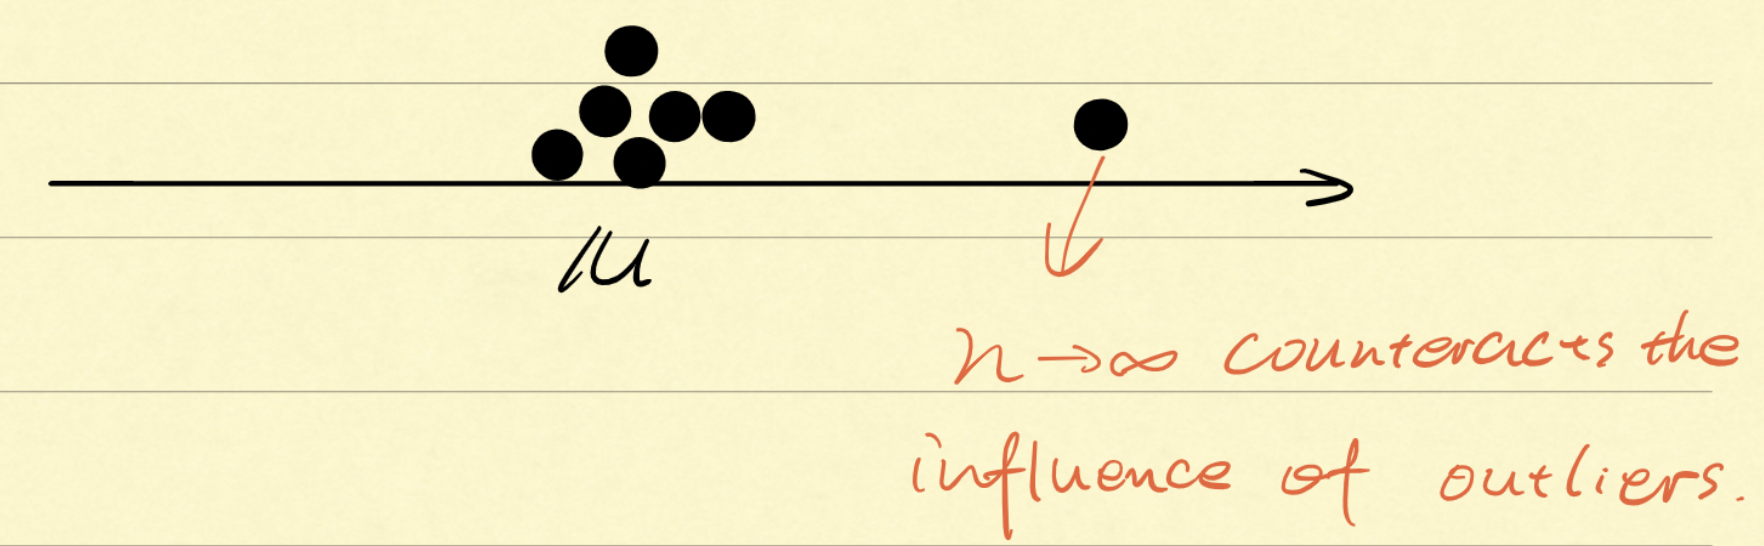
\includegraphics[scale=0.3]{wLLN.png}
        \caption{convergence in probability}
        \label{}
    \end{figure}\end{center}
    \item Strong Law of Large Numbers (sLLN)
    $$P(|\bar{x}-\mu|\geq\varepsilon\text{ as }n \rightarrow+\infty)=0,\ \forall \varepsilon>0$$
    \begin{center}\begin{figure}[htbp]
        \centering
        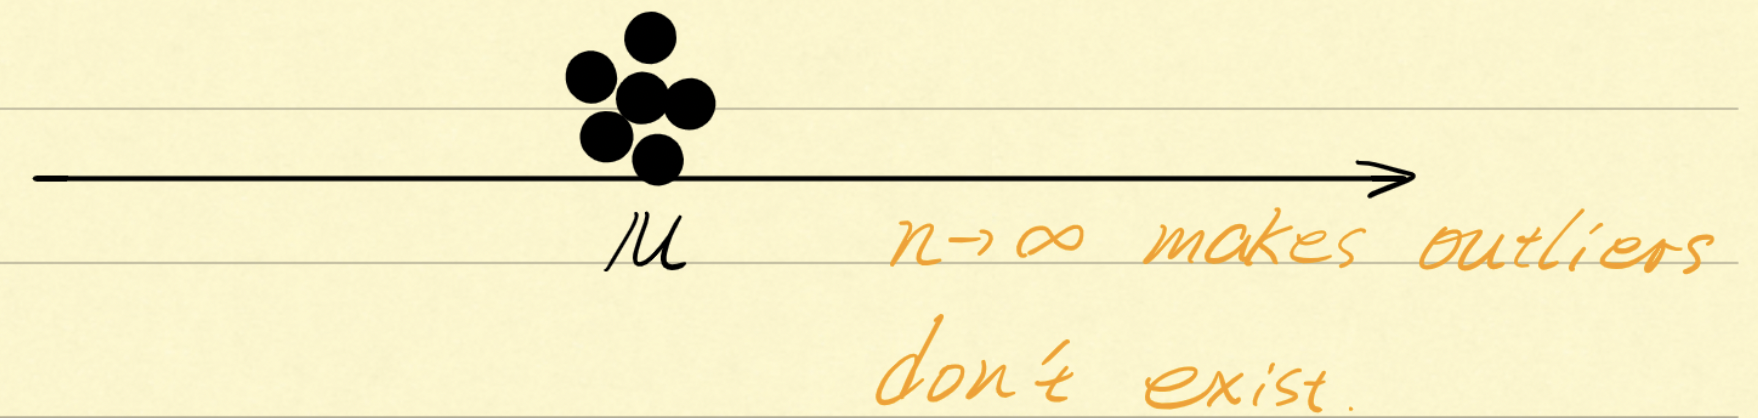
\includegraphics[scale=0.3]{sLLN.png}
        \caption{wp1(a.s.)}
        \label{}
    \end{figure}\end{center}
\end{enumerate}

\subsection{Central Limit Theorem (CLT)}
\begin{theorem}[Central Limit Theorem (CLT)]
    $$Z=\frac{\overline{X}-\mu}{\frac{\sigma}{\sqrt{n}}} \xrightarrow {D} N(0,1) \text{ when}\ n\to \infty$$
    $Z$ \underline{converges in distribution} to $N(0,1)$ as $n\to \infty$

    (converges in distribution: $P(\frac{\overline{X}-\mu}{\frac{\sigma}{\sqrt{n}}}\leq a)\rightarrow \frac{1}{\sqrt{2\pi}}\int_{-\infty}^ae^{-\frac{x^2}{2}}dx$)
\end{theorem}
\begin{proof}
    Prove the situation of $\mu=0,\sigma^2=1$, we can use linear transformations to get other situations.

    Moment-generating function(MGF) of $X_i$: $M_0(t)=E(e^{tX_i})$. $$M_0(0)=1,M_0'(0)=EX_i=0,M_0''(0)=EX_i^2=1$$
    Moment-generating function(MGF) of $\sqrt{n}\overline{X}$:
    \begin{equation}
        \begin{aligned}
            M_1(t)&=Ee^{t\sqrt{n}\overline{X}}=Ee^{t\frac{\sum_{i=1}^nX_i}{\sqrt{n}}}\\
            &=Ee^{t\frac{X_1}{\sqrt{n}}}\cdot Ee^{t\frac{X_2}{\sqrt{n}}}\cdots Ee^{t\frac{X_n}{\sqrt{n}}}\\
            &=[M_0(\frac{t}{\sqrt{n}})]^n
        \end{aligned}
        \nonumber
    \end{equation}
    \begin{equation}
        \begin{aligned}
            \lim_{n \rightarrow	\infty}\log M_1(t)&=\lim_{n \rightarrow	\infty}n\log M_0(\frac{t}{\sqrt{n}})\\
            &(\text{let }y=\frac{1}{\sqrt{n}})\\
            &=\lim_{y=0}\frac{\log M_0(yt)}{y^2}\\
            &(\text{L'Hôpital's rule})\\
            &=\lim_{y=0}\frac{t M'_0(yt)}{2y M_0(yt)}\\
            &(\text{L'Hôpital's rule})\\
            &=\lim_{y=0}\frac{t^2 M''_0(yt)}{2 M_0(yt)+2ytM'(yt)}\\
            &=\frac{t^2}{2}
        \end{aligned}
        \nonumber
    \end{equation}
    As we know the Moment-generating function(MGF) of $Z\sim N(0,1)$ is $M_Z(t)=\frac{t^2}{2}$.

    Hence, $M_1(t)=M_Z(t)$ i.e. $\frac{\overline{X}-\mu}{\frac{\sigma}{\sqrt{n}}} \xrightarrow {D} N(0,1)$ as $n \rightarrow\infty$
\end{proof}



\section{Markov Chain}
\subsection{Definition}
For discrete state space $S$, a Markov Chain is a stochastic process $X_0,X_1,X_2,...$   such that$$P(X_{n+1}=i|X_n=j,X_{n-1}=x_{n-1},...,X_0=x_0)=P(X_{n+1}=i|X_n=j)$$
for all $n\in \mathbb{Z}$ and $x_0,x_1,...,x_{n-1},i,j\in S$.

A MC is called \underline{time homogeneous} if $P(X_{n+1}=i|X_n=j)=P(X_1|X_0=j),\forall n\in \mathbb{Z}^+$ and $i,j\in S$ (we only consider time homogeneous MC).

The \textbf{transition probabilities} for a \underline{time homogeneous MC} can be written down as a matrix $P$ satisfying $P_{ij} = P (X_1 = j|X_0 = i)$. This matrix $P$ satisfies two properties:
\begin{enumerate}[(1)]
    \item $P_{ij}\geq 0$ for all $i,j\in S$.
    \item $\sum_{j\in S}P_{ij}=1$ for all $i\in S$.
\end{enumerate}
Any matrix satisfies the two properties is called a \textbf{stochastic matrix}.

\subsection{Matrix Computations}
Given a time homogeneous MC with initial distribution $X_0\sim\alpha\in [0,1]^{|S|}$ and transition matrix $P$.
\begin{lemma}[Distribution of Entire Sequence]
$$P(X_0=x_0,X_1=x_1,...,X_n=x_n)=P(X_0=x_0)P_{x_0,x_1}P_{x_1,x_2}...P_{x_{n-1},x_n}$$
\end{lemma}

\begin{lemma}[Markov Property]
    $$P(X_{t_n}=x_{t_n} | X_{t_{n-1}}=x_{t_{n-1}},...,X_{t_0}=x_{t_0})=P(X_{t_n}=x_{t_n}|X_{t_{n-1}}=x_{t_{n-1}})$$
\end{lemma}

\begin{lemma}[Transition Probability after $n$ states]
$$P(X_n=j|X_0=i)=(P^n)_{ij}$$
\end{lemma}
\begin{proof}
    $P(X_2=j|X_0=i)=\sum_{k\in S}P(X_2=j|X_1=k)P(X_1=k|X_0=i)=\sum_{k\in S}P_{kj}P_{ik}=(P^2)_{ij}$. Then prove by mathematical induction,
    $P(X_n=j|X_0=i)=\sum_{k\in S}P(X_n=j|X_{n-1}=k)P(X_{n-1}=k|X_0=i)=\cdots =(P^n)_{ij}$
\end{proof}

\subsubsection{Chapman Kolmogorov Equations (C-K Equations) $P(X_{n+m}=j|X_0=i)=(P^{m+n})_{ij}=\sum_{k\in S}(P^{m})_{ik}(P^{n})_{kj}$}
$m-$step transition probabilities from state $k$ to state $j$:
\begin{equation}
    P(X_{n+m}=j|X_0=i)=(P^{m+n})_{ij}=\sum_{k\in S}(P^{m})_{ik}(P^{n})_{kj}
\end{equation}
\begin{proof}
    $P(X_n=j|X_0=i)=\sum_{k\in S}P(X_{n+m}=j|X_{m}=k)P(X_{m}=k|X_0=i)=\sum_{k\in S}P(X_n=j|X_{0}=k)P(X_{m}=k|X_0=i)$
\end{proof}

\subsubsection{Marginal Distribution $P(X_n=j)=(\alpha P^n)_{j}$}
\begin{lemma}[Marginal Distribution]
    Given initial distribution $X_0\sim\alpha$ and transition matrix $P$. $\alpha$ is distribution vector ($1\times|S|$) with $\sum_{i\in S}{\alpha_i}=1$.
    $$P(X_n=j)=(\alpha P^n)_{j}$$
\end{lemma}
\begin{corollary}[Distribution of Subsequence]
    $$P(X_{t_{n}}=x_{t_{n}},X_{t_{n-1}}=x_{t_{n-1}},...,X_{t_0}=x_{t_0})=(\alpha P^{t_0})_{x_{t_0}}P^{t_1-t_0}_{x_{t_0},x_{t_1}}P^{t_2-t_1}_{x_{t_1},x_{t_2}}\cdots P^{t_{n}-t_{n-1}}_{x_{t_{n-1}},x_{t_{n}}}$$
\end{corollary}

\subsection{States}
\begin{enumerate}[$\bullet$]
    \item \underline{Accessible}: $j$ is accessible from $i$ if $\exists n$ s.t. $P_{ij}^n>0$.
    \item \underline{Communicate/Communication}: $i$ communicates $j$ ($i \leftrightarrow j$) if $j$ is accessible from $i$ and $i$ is accessible from $j$. (Reflexivity: $i \leftrightarrow i$; Symmetry: $i \leftrightarrow j$ $\Rightarrow$ $j \leftrightarrow i$; Transitivity: $i \leftrightarrow j$ and $j \leftrightarrow k$ $\Rightarrow$ $i \leftrightarrow k$.)
    \item \underline{Class}: if $i \leftrightarrow j$, then states $i,j$ are said to be in the same \underline{(communication) class}. (Since communication is an equivalence relation, the state space can be partitioned into equivalence classes, called \textit{communication classes}.)
    \item \underline{Irreducible}: A Markov Chain that has \underline{only one class} is said to be \underline{irreducible}.
    \item \underline{Recurrent}: State $i$ is recurrent if $f_i=P($ever re-enter state $i$ if started in state $i)=1$. (the expected number of times it visits state $i$ is $\sum_{n=0}^\infty P_{ii}^n=+\infty$). (A MC is irreducible if all states are recurrent)
    \item \underline{Transient}: State $i$ is transient if $f_i=P($ever re-enter state $i$ if started in state $i)<1$. (the expected number of times it visits state $i$ is $\sum_{n=0}^\infty P_{ii}^n<+\infty$; $P($visits state $i$ exactly $n$ times$)=f_i^{n-1}(1-f_i)$; The expected number is $\sum_{n=0}^\infty f_i^n(1-f_i)n={n=0}^\infty P_{ii}^n<\infty$).
    
    (A communicating class is called transient if starting from that class, with probability $1$ the MC leaves that class and never returns. The states of such a class are called transient states.)
    \begin{lemma}
        If $i$ is recurrent, $i\leftrightarrow j \Rightarrow$ $j$ is recurrent.
    \end{lemma}
    \begin{theorem}
        The states of a communication class are \underline{either all recurrent or all transient}.
    \end{theorem}
    \begin{corollary}
        For a \underline{finite irreducible} Markov chain, all states are recurrent.
    \end{corollary}
\end{enumerate}

\subsubsection*{Canonical Decomposition}
\begin{definition}
    A set of states $C$ is said to be \underline{closed} if no state outside of $C$ is accessible from any state in $C$. If $C$ is closed, then $$P_{ij} = 0,\ \forall i\in C,j\notin C$$
\end{definition}

\begin{lemma}
    (1) A communication class is \underline{closed} if it consists of all recurrent states.
    (2) A finite communication class is closed only if it consist of all recurrent states.
\end{lemma}
\begin{proof}
(1): if not closed, $\exists i\in C,j\notin C, P_{ij}>0$. $i$ shouldn't be accessible from $j$ since $i,j$ are not in one class. There exists positive probability that starting from $i$ then hit $j$ and never hit $i$ again, which contradicts to $i$ is recurrent. (2):According to former corollary, a finite class's all states are recurrent.
\end{proof}

\subsection{Periodicity}
Suppose $P$ is the transition matrix for an irreducible MC. For a given state $i$, we define the set $$J_i=\{n\geq 1:P^n(i,j)>0\}$$
$J_i$ is the set of times when it is possible for the MC to come back to $i$ starting from $i$ at time $0$. We define the \textbf{period} of a state $i$ is $$d(i)=gcd(J_i)$$
\subsubsection{Lemma: all states in an irreducible MC have the same period}
\begin{lemma}
    For an irreducible MC, all states have the same period.
\end{lemma}
\begin{proof}
    Let $d$ be a common divisor of $J_i$. Consider any other state $j$. We want to show $d$ is also the common divisor of $J_j$.
    
    Since the MC is irreducible, there exists $m$ and $n$ s.t. $P_{ij}^m>0$ and $P_{ji}^n>0$. Then $P_{ii}^{m+n}\geq P_{ij}^mP_{ji}^n >0 \Rightarrow m+n\in J_i$. $d$ should be a divisor of $m+n$.

    For any $l\in J_j$, $P_{ii}^{m+n+l}\geq P_{ij}^mP_{jj}^lP_{ji}^n >0 \Rightarrow m+n+l\in J_i$. $d$ divides $m+n+l$ $\Rightarrow$ $d$ divides $l$. Since $l$ can be any number in $J_j$, $d$ is a common divisor of $J_j$.
\end{proof}

\subsubsection{Periodic, Aperiodic}
A \underline{state} is \textbf{aperiodic} if period equals $1$, \textbf{periodic} otherwise.\\
A \underline{chain} is \textbf{aperiodic} if \underline{all} its states are aperiodic, \textbf{periodic} otherwise.

\subsection{Regular Matrix}
\subsubsection{Regular matrix: $\exists n\geq 1$ s.t. $P^n>0$}
A matrix $M$ is said to be positive if all the entries of $M$ are positive. We write $M > 0$.
\begin{definition}[Regular Transition Matrix]
    A transition matrix $P$ is said to be \underline{regular} if some power of $P$ is positive. That is, $P^n >0$, for some $n\geq 1$.
\end{definition}

\subsubsection{Theorem}
\begin{theorem}
    A MC with transition matrix $P$, then for some $n\geq 1$ $$P^n_{ii}>0,\forall i$$
\end{theorem}

\subsubsection{Lemma: Finite MC is Irreducible, Aperiodic $\Leftrightarrow$ has Regular transition matrix}
\begin{lemma}
    A finite MC is \textbf{irreducible} and \textbf{aperiodic} is equivalent to the transition matrix $P$ is \textbf{regular}.
\end{lemma}

\subsection{Long Run Behavior of Finite Markov Chains}
As $n \rightarrow \infty$, $P^n$:
\begin{enumerate}[(1)]
    \item Convergence. ($P^{n+1}=P^n$)
    \item Forgetting the initial states. (each row is identical)
\end{enumerate}

\subsubsection{Limiting Distribution}
\begin{definition}
    A MC is said to have a \textbf{limiting distribution} $\lambda$ if we have $$\lim_{n \rightarrow \infty}P_{ij}^n=\lambda_j,\ \forall i,j\in S$$
    An \underline{equivalent definition} is that for all initial distributions $X_0\sim \alpha$ and all $j\in S$ we have
    $$\lim_{n \rightarrow \infty}(\alpha P^n)_j=\lambda_j$$
\end{definition}

\textbf{Example: }$P=\begin{bmatrix}
    1-p&p\\
    q&1-q
\end{bmatrix}$. If $p+q=1$, each rows of $P$ is the same and $P^n=P$.

Assume $p+q\neq 1$,
\begin{equation}
    \begin{aligned}
        P^n_{11}&=P^{n-1}_{11}(1-p)+P^{n-1}_{12}q\\&=P^{n-1}_{11}(1-p)+(1-P^{n-1}_{11})q\\
        P^n_{11}&=\frac{q}{p+q}+\frac{p}{p+q}(1-p-q)^n \rightarrow \frac{q}{p+q}\text{ as }n \rightarrow \infty\\
        \lim_{n \rightarrow \infty}P^n&=\frac{1}{p+q}\begin{bmatrix}
            q&p\\
            q&p
        \end{bmatrix}
    \end{aligned}
    \nonumber
\end{equation}

\begin{lemma}
    If $\lambda$ is the limiting distribution for a MC with transition matrix $P$ then $\lambda$ satisfies the equation $$\lambda P=\lambda$$
\end{lemma}
\begin{proof}
    $(\lambda P)_j=\sum_{i\in S}\lambda_i P_{ij}=\sum_{i\in S}\lim_{n \rightarrow \infty}P_{ki}^nP_{ij}=\lim_{n \rightarrow \infty}\sum_{i\in S}P_{ki}^nP_{ij}=\lim_{n \rightarrow \infty}P_{kj}^{n+1}=\lambda_j$
\end{proof}

\subsubsection{Stationary Distribution}
\begin{definition}
    A distribution $\pi$ which satisfies the equation $$\pi P=\pi$$ is called a \textbf{stationary distribution} for the MC.
\end{definition}
\textbf{Note: }A limiting distribution $\lambda$ for the MC has to also be a stationary distribution. The converse is not always true.



\subsubsection{Limiting Distribution: expected proportion of time in each state}
The entries of the limiting distribution can also be interpreted as \textbf{the limit of the expected proportion of time the MC spends in each of the corresponding states.} For any state $j$, define the indicator random variable $I_k=1(X_k=j)$. Now define $$F_{n,j}=\frac{1}{n}\sum_{k=0}^{n-1}I_k$$
The random variable $F_{n,j}$ represents the proportion of time till time $n-1$ the MC spends in state $j$.

\begin{lemma}
    If $\lambda$ is the limiting distribution for a MC with transition matrix $P$ then $\lambda$ satisfies the equation $\lim_{n \rightarrow \infty}\mathbb{E}(F_{n,j}|X_0=i)=\lambda_j$ for all $j,i\in S$
\end{lemma}
\begin{proof}
    We can write $$\mathbb{E}(F_{n,j}|X_0=j)=\mathbb{E}\frac{1}{n}\sum_{k=0}^{n-1}\mathbb{E}(I_k|X_0=i)=\frac{1}{n}\sum_{k=0}^{n-1}P(X_k=j|X_0=i)=\frac{1}{n}\sum_{k=0}^{n-1}P_{ij}^k$$
    Therefore, taking limits we can conclude that $$\lim_{n \rightarrow \infty}\mathbb{E}(F_{n,j}|X_0=j)=\lim_{n \rightarrow \infty}\frac{1}{n}\sum_{k=0}^{n-1}P_{ij}^k=\lim_{n \rightarrow \infty}P_{ij}^n=\lambda_j$$
\end{proof}

\subsubsection{Fundamental Theorem for Irreducible, Aperiodic, Finite MC: $\exists$ unique limiting distribution $\pi$ and $\pi_j>0,\forall j$}
\begin{theorem}
    If $P$ is the transition matrix for an irreducible, aperiodic (finite) Markov chain then there exists a unique stationary distribution or a unique solution to the equation $\pi=\pi P$ which satisfies the following two properties:
    \begin{enumerate}[(1)]
        \item $\pi$ is the \textbf{limiting distribution} of the MC. ($\lim_{n \rightarrow \infty}\alpha P^n=\pi,\forall \alpha$ initial distribution)
        \item $\pi$ gives \textbf{positive} probability to each of the states. ($\pi_j>0,\forall j\in S$)
    \end{enumerate}
\end{theorem}

\subsubsection{Limit Theorem for Finite Irreducible Markov Chains}
$T_j=\min\{n>0 : X_n = j\}$ is the first passage time to state $j$.
\begin{theorem}
    Assume that $X_0, X_1,...$ is an \underline{finite irreducible} Markov chain. For each state $j$, let $\mu_j = \mathbb{E}(T_j|X_0 = j)$ be the expected return time to $j$. Then, $\mu_j$ is finite, and there exists a unique positive stationary distribution $\pi$ such that $$\pi_j=\frac{1}{\mu_j},\forall j$$
    Furthermore, for all states $i$, $$\pi_j=\lim_{n \rightarrow \infty}\frac{1}{n}\sum_{m=0}^{n-1}P_{ij}^m$$
\end{theorem}














\end{document}